\section{1174050 Dika Sukma Pradana}
\subsection{Teori}
\begin{enumerate}
\item Definisi, sejarah, dan perkembangan kecerdasan buatan.
\subitem Intelegensi buatan (AI) mengacu pada simulasi kecerdasan manusia dalam mesin yang diprogram untuk berpikir seperti manusia dan meniru tindakan mereka. Istilah ini juga dapat diterapkan pada mesin apa pun yang menunjukkan sifat-sifat yang terkait dengan pikiran manusia seperti pembelajaran dan pemecahan masalah.
\subitem Sejarah Kecerdasan Buatan (AI) bermula pada saat zaman kuno, dengan sejuta mitos, cerita dan desas-desus tentang makhluk buatan yang diberkahii dengan kecerdasan oleh pengrajin ahli. Benih-benih AI modern ditanam oleh para filsuf klasik yang mencoba menggambarkan proses pemikiran manusia sebagai manipulasi simbol secara mekanis. Karya ini memuncak dalam penemuan komputer digital yang dapat diprogram pada tahun 1940-an, sebuah mesin yang didasarkan pada esensi abstrak penalaran matematika. Perangkat ini dan ide-ide di belakangnya menginspirasi segelintir ilmuwan untuk mulai serius membahas kemungkinan membangun otak elektronik.
Bidang penelitian AI didirikan pada lokakarya yang diadakan di kampus Dartmouth College selama musim panas 1956. Mereka yang hadir akan menjadi pemimpin penelitian AI selama beberapa dekade. Banyak dari merekka meramaIkan bahwa sebuah mesin yang secerdas manusia akan hidup tidak lebih dari satu generasi dan mereka diberi jutaan dolar untuk mewujudkan visi atau tujuan ini.
Akhirnya, menjadi jelas bahwa mereka meremehkan kesulitan proyek. Pada tahun 1973, sebagai tanggapan atas kritik dari James Lighthill dan tekanan terus-menerus dari kongres, AS dan Pemerintah Inggris menghentikan pendanaan penelitian yang tidak diarahkan pada kecerdasan buatan, dan tahun-tahun sulit berikutnya akan dikenal sebagai musim dingin AI. Tujuh tahun kemudian, sebuah inisiatif visioner oleh Pemerintah Jepang mengilhami pemerintah dan industri untuk menyediakan miliaran dolar dalam AI, tetapi pada akhir 80-an investor menjadi kecewa dengan kurangnya daya komputer (perangkat keras) yang dibutuhkan dan menarik lebih banyak dana.
Investasi dan minat pada AI tumbuh pesat pada dekade pertama abad ke-21, ketika pembelajaran mesin berhasil diterapkan pada banyak masalah di dunia akademis dan industri karena metode baru, penerapan perangkat keras komputer yang kuat, dan kumpulan data yang sangat besar.
\item  Definisi supervised learning, klasifikasi, regresi, dan unsupervised learning. Data set, training set dan testing set. 
\subitem Supervised learning adalah sebuah metode pendekatan yang mana sudah terdapat data yang dilatiih, dan terdapat variabel yang ditargetkan atau yang menjadi tujuan sehingga tujuan dari pendekatan ini adalah mengkelompokan suatu data ke data yang sudah ada. Sedangkan unsupervised learrning tidak memiliki data latiih, sehinggga dari data yang ada, kita mengelompokan data tersebbut menjadi dua bagian atau bahkan tiga bagian dan seterusnya.
\subitem Klasifikasi adalah salah satu topik utama dalam data mining atau machine learning. Klasifikasi yaitu suatu pengelompokan data dimana data yang digunakan tersebut mempunyai kelas label atau target.
\subitem Regresi adalah Supervised learning tidak hanya mempelajari classifier, tetapi juga mempelajari fungsi yang dapat memprediksi suatu nilai numerik. 
\subitem Data set merupakan sebuah cabang aplikasi dari Artificial Intelligence(AI)/Kecerdasan Buatan yang terfokus kepada pengembangan sebuah sistem yang mampu belajar sendiiri tannpa harus berulang kalai di program oleh manusia(programmer).
\subitem Training set yaitu jika pasangan objek, dan kelas yang menunjuk pada objek tersebut adalah suatu contoh yang telah diberi label akan menghasilkan suatu algoritma pembelajaran.
\subitem Testing set digunakan untuk mengukur sejauh mana classifier berhasil melakukan klasifikasi dengan benar\cite{zhu2009introduction}.
\end{enumerate}

\subsection{Instalasi}
\subsubsection{Instalasi Library Scikit dari Anaconda}
\begin{enumerate}
\item Download aplikasi Anaconda terlebih dahulu. 
\item Install aplikasi Anaconda yang sudah di download tadi. 
\item Simpan aplikasi sesuai folder yang kita pilih lalu next. 
\item Centang Keduanya lalu tekan tombol install. 
\item Setelah itu tunggu sampai proses instalasi selesai lalu jika sudah tekan tombol finish. 
\item Lalu buka command prompt anda dan tuliskan perintah berikut ini untuk mengecek apakah aplikasinya sudah terinstall. 
\item Kemudian ketikkan perinta pip install -U scikit-learn seperti gambar berikut. 
\end{enumerate}
         \begin{figure}[H]
                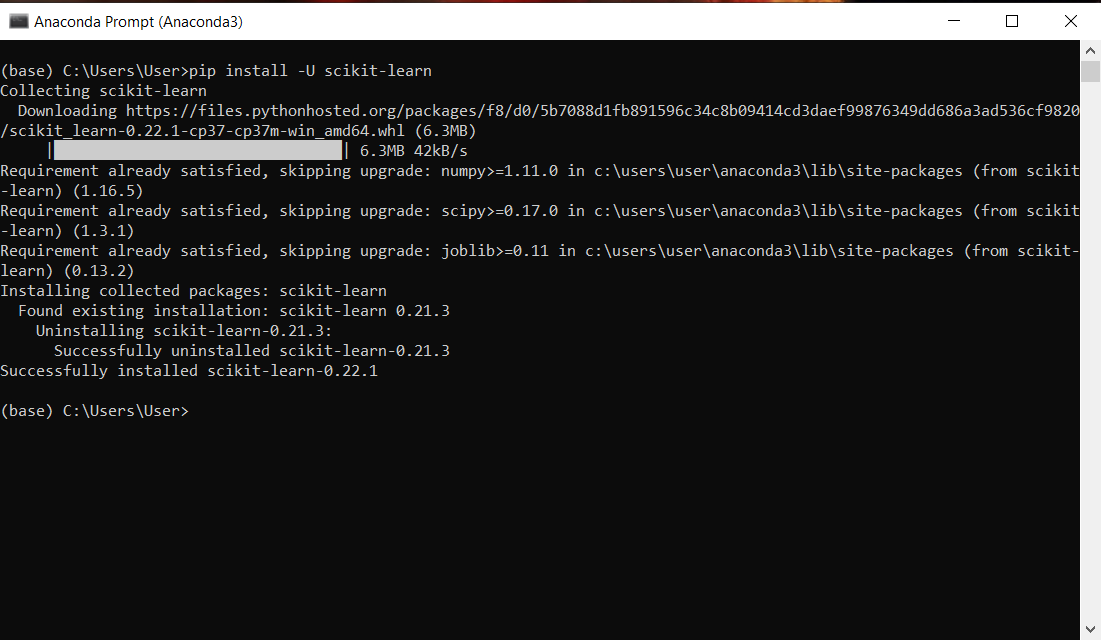
\includegraphics[width=4cm]{figures/1174050/chapter1/instal.png}
                \centering
                \caption{Instalasi}
            \end{figure}


\subsection{Percobaan}
Mencoba Library
\lstinputlisting{src/1174050/chapter1/VAR.py}
 \begin{figure}[H]
                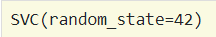
\includegraphics[width=4cm]{figures/1174050/chapter1/2.png}
                \centering
                \caption{Variabel Explore}
            \end{figure}


\subsubsection{Mencoba Loading an example Dataset}
\lstinputlisting{src/1174050/chapter1/dataset.py}
 \begin{figure}[H]
                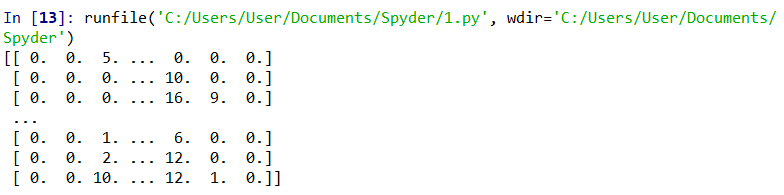
\includegraphics[width=4cm]{figures/1174050/chapter1/1.png}
                \centering
                \caption{Datasets}
            \end{figure}


\subsubsection{Learning and Predicting}
\lstinputlisting{src/1174050/chapter1/learning.py}


\subsubsection{Model Presistence}
\lstinputlisting{src/1174050/chapter1/modelpersistance.py}


\subsubsection{Conventions}
Type Casting
\lstinputlisting{src/1174050/chapter1/typecasting.py}
Refitting and updating parameters
\lstinputlisting{src/1174050/chapter1/Multiclass.py}
Multiclass vs. multilabel fitting
\lstinputlisting{src/1174050/chapter1/Refitting.py}


\subsection{Penanganan eror}
\subsubsection{ScreenShoot Eror}
\begin{figure}[ht]
\centering
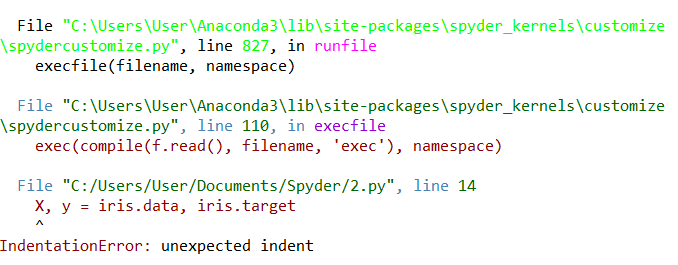
\includegraphics[scale=0.5]{figures/1174050/chapter1/error.png}
\caption{Error}
\label{contoh}
\end{figure}

\subsubsection{Tuliskan Kode Eror dan Jenis Erornya}
\begin{verbatim}
IndentationError: unexpected indent
\end{verbatim}


\subsubsection{Solusi Pemecahan Masalah Error}
Pastikan semua spasi pada koding sama. Menggunakan spasi atau tab.

\subsection{Plagiarism}
    \begin{figure}[H]
        \centering
        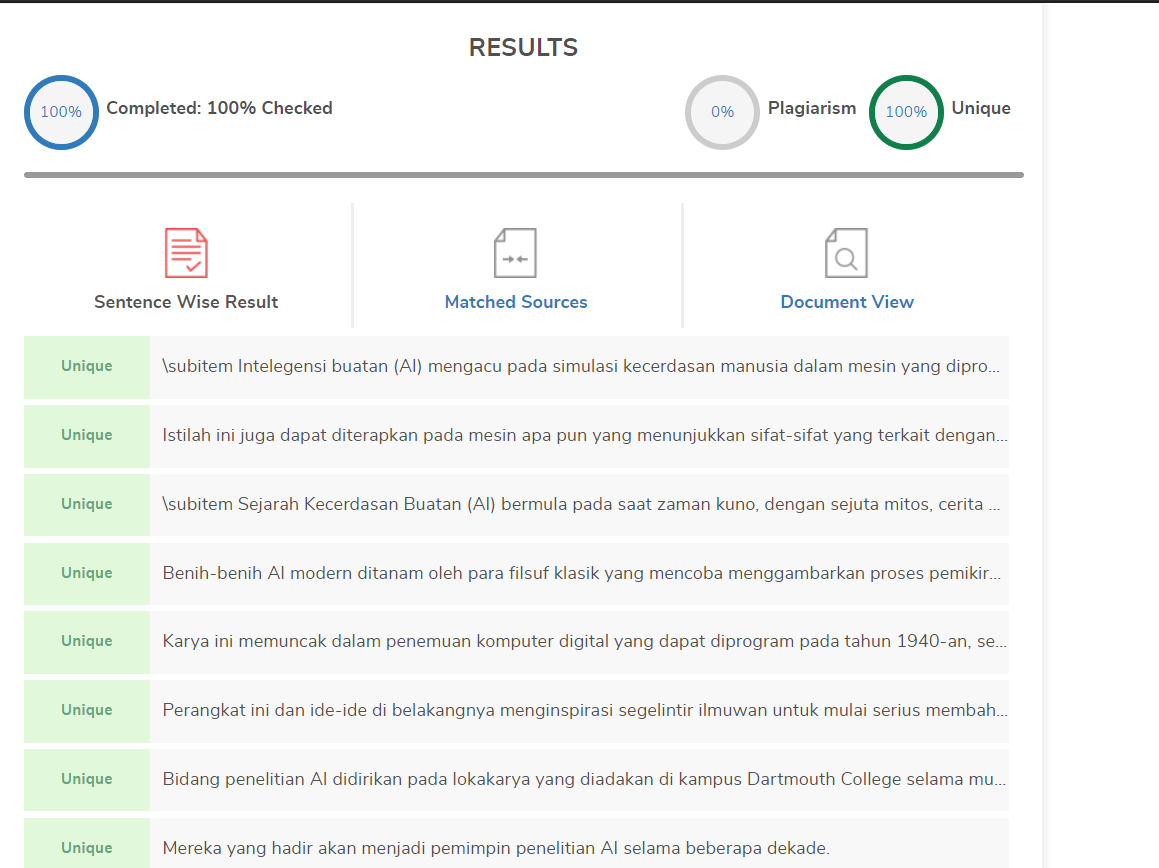
\includegraphics[width=1\textwidth]{figures/1174050/chapter1/plagiarism.png}
        \caption{Plagiarism}
        \label{print}
    \end{figure}